\input{def}
\pagestyle{empty}
\begin{document}

\begin{center}
\large{ MATH-6890 \hspace{1in} Numerical Solutions of Waves  \hspace{1in}Fall 2016 \\ Due Monday October 3, 2016.}\end{center}
Michael Hennessey

\bigskip
\bc {\bf Problem Set 4} \ec
\benum 

\item Use the ansatz $u=\exp(ikx)$ to determine approximations to $u_x$ with order of accuracy from 2 and 10:
$$ u_{x,j}=\left[D_0\sum_{m=0}^\infty \alpha_m\Delta x^{2m}(D_+D_-)^m\right]u_j.$$
Plot the real part of the symbols of the resultant 5 discretizations on a single plot, and plot the imaginary part of the symbol for the resultant 5 discretizations on a separate plot. In each case, include the symbol of the exact operator as well. Make a separate set of 2 plots showing the error in the real and imaginary parts for the various schemes. Discuss.\\

Solution:\\

The approximation has the symbol
$$i\xi =i \sin(\xi)\sum_{m=0}^\infty \alpha_m[-4\sin^2(\xi/2)]^m$$
which becomes slightly nicer if we make the substitution $2\eta = \xi$:
$$2i\eta = \sin(2\eta)\sum_{m=0}^\infty \alpha_m[-4\sin^2(\eta)]^m.$$
where the $\alpha_m$ were found using the maple script ``D0Example.mw'' located on your webpage. We have
$$\alpha_0=1,\;\;\alpha_1 = -\frac{1}{6},\;\; \alpha_2 = \frac{1}{30},\;\; \alpha_3 = -\frac{1}{140},\;\; \alpha_4 = \frac{1}{630}.$$
Thus the symbols for the 2nd-10th order accuracy may be found from the truncation of the expression below to the appropriate number of terms (i.e., 2nd order = 1 term, 4th order = 2 terms, etc...)
$$2i\eta = i\sin(2\eta)\left[1+\frac{2}{3}\sin^2(\eta)+\frac{8}{15}\sin^4(\eta)+\frac{16}{35}\sin^6(\eta)+\frac{128}{315}\sin^8(\eta)\right].$$
\begin{figure}[h]
\centering
\includegraphics[width=2.5in]{real_sym1}
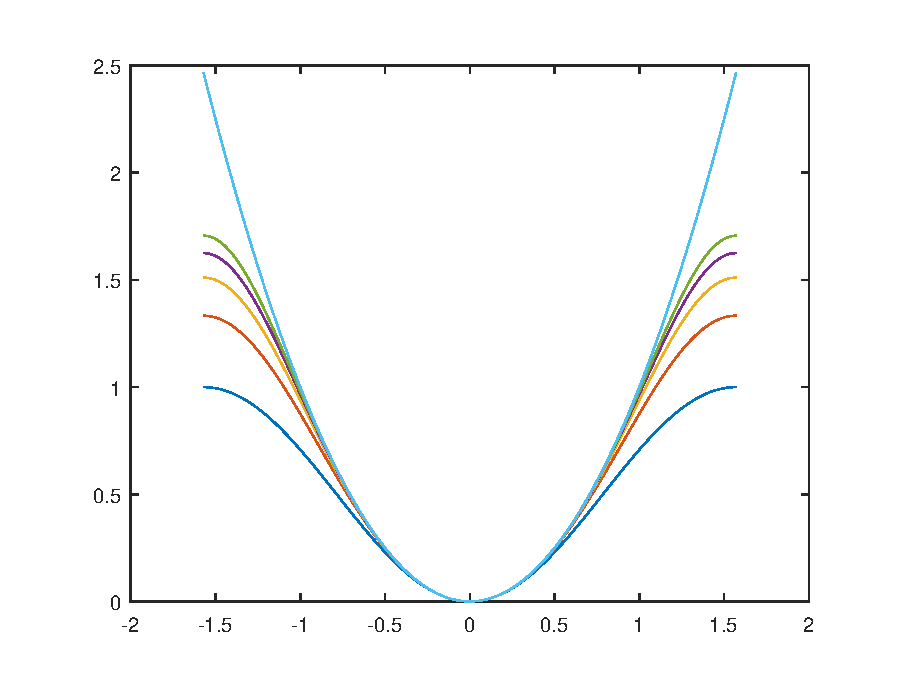
\includegraphics[width=2.5in]{real_err1}
\end{figure}
The plots of the symbols are included here.\\
Clearly, we can see that the real part of this operator is 0. We also see that the error grows exponentially as the symbol attempts to go back to zero near the bound $\eta = \pm\pi/2$ for all orders of accuracy examined. Thus we can see that this operator is unstable, especially if we are concerned with the $\pm$ mode, or other similar modes near $\eta = \pm \pi/2.$ However, we do still get some nice behavior on the interior of the modes (say from $\eta=-\pi/4$ to $\eta=\pi/4$) as the order of accuracy is extended.
\begin{figure}[ht]
\centering
\includegraphics[width=3in]{imag_sym1}
\includegraphics[width=3in]{imag_err1}
\end{figure}

\item Do the same as 1., but with 
$$u_{xx,j}=\left[D_+D_-\sum_{m=0}^\infty \delta_m\Delta x^{2m}(D_+D_-)^m\right]u_j.$$

Solution:\\

The approximation has the symbol
$$-\xi^2 = -4\sin^2(\xi/2)\sum_{m=0}^\infty \delta_m[-4\sin^2(\xi/2)]^m.$$
We make the substitution $2\eta=\xi$ to get
$$-4\eta^2 = -4\sin^2(\eta)\sum_{m=0}^\infty\delta_m[-4\sin^2(\eta)]^m.$$

We use the same script as before to find the constants
$$\delta_0=1,\;\; \delta_1 = -\frac{1}{12},\;\;\delta_2 = \frac{1}{90},\;\;\delta_3 = -\frac{1}{560},\;\;\delta_4 = \frac{1}{3150}.$$

Then the symbols at 2nd-10th order accuracies may be found by the truncation of the expression below to the appropriate number of terms:
$$\eta^2=\sin^2(\eta)\left[1+\frac{1}{3}\sin^2(\eta)+\frac{8}{45}\sin^4(\eta)+\frac{4}{35}\sin^6(\eta)+\frac{128}{1575}\sin^8(\eta)\right].$$
The plot of the symbol and the errors may be found at the beginning of the next page. We can see that the imaginary parts of this operator (both symbol and error) are zero. We also see that the error remains small and is lessened substantially by each higher order of approximation.
\pagebreak
\begin{figure}[ht]
\centering
\includegraphics[width=3in]{real_sym2}
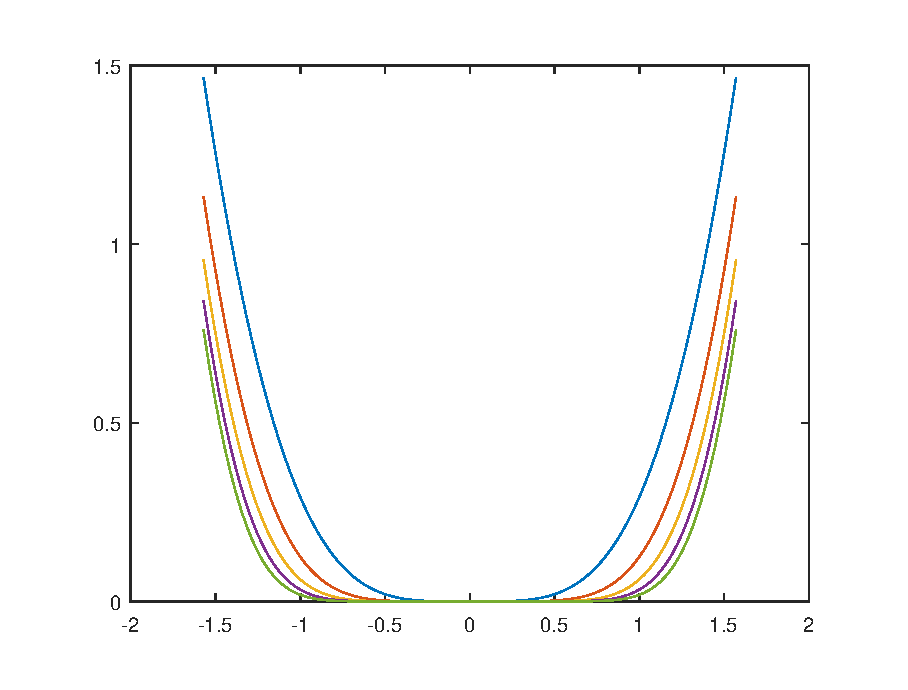
\includegraphics[width=3in]{real_err2}\\
\includegraphics[width=3in]{imag_sym2}
\includegraphics[width=3in]{imag_err2}
\end{figure}

\item Consider the wave problem
\begin{align*}
u_{tt}&=c^2u_{xx},\;\;\; t\geq 0,\;\; 0\leq x\leq 1,\\
u(x,0)&=f(x)\\
u_t(x,0)&=g(x)\\
u_x(0,t)&=u(1,t)=0.
\end{align*}

\benum
\item Use the modified equation time stepper 
$$\frac{u_j^{n+1}-2u_j^n+u_j^{n-1}}{\Delta t^2}=(u_{tt})_j^n+\frac{\Delta t^2}{12}(u_{tttt})_j^n+O(\Delta t^4)$$
to construct a 4th order accurate discretization in space and time on the grid $x_j=j\Delta x, 0\leq j\leq N,\Delta x=1/N.$ Use compatibility BCs to define the solution in ghost cells.\\
Solution:\\
We first rewrite the modified equation time stepper in terms of spatial derivatives:
$$u_j^{n+1}=2u_j^n-u_j^{n-1}+\Delta t^2 c^2 (u_{xx})_j^n+\frac{\Delta t^4 c^4}{12}(u_{xxxx})_j^n.$$
Then we make the appropriate 4th order approximation to $u_{xx}$ and 2nd order approximation to $u_{xxxx}$:
\begin{multline*}
u_j^{n+1}=2u_j^n-u_j^{n-1}+\frac{c^2\Delta t^2}{12\Delta x^2}[-u_{j-2}^n+16u_{j-1}^n-30u_j^n+16u_{j+1}^n-u_{j+2}^n]\\
+\frac{c^4\Delta t^4 }{12\Delta x^4}[u_{j-2}^n-4u_{j-1}^n+6u_j^n-4u_{j+1}^n+u_{j+2}^n].
\end{multline*}
We then let $\frac{c\Delta t}{\Delta x}=\l$ for future ease of use.\\
\par Now we address the ghost cells. First at the left, with the Neumann condition, with $j=-2,1$. We first find the 4th order approximation to the first derivative:
$$u_x(0,t)=0\;\;\implies\;\; \frac{1}{12\Delta x}[u_{-2}^n-8 u_{-1}^n+8u_{1}^n-u_{2}^n]=0.$$
After some simplification, this becomes
$$u_{-2}^n-8 u_{-1}^n=-8u_{1}^n+u_{2}^n.$$
We then differentiate twice in time to find a compatibility condition on the third spatial derivative at 0, and use the 2nd order approximation of that derivative.
$$u_x(0,t)=0\;\;\implies\;\; u_{xtt}(0,t)=c^2u_{xxx}(0,t)=0$$
$$u_{xxx}(0,t)=0\;\;\implies\;\; \frac{1}{2\Delta x^3}[-u_{-2}^n+2u_{-1}^n-2u_{1}^n+u_{2}^n]=0.$$
Which simplifies to
$$-u_{-2}^n+2u_{-1}^n=2u_{1}^n-u_{2}^n.$$
These equations are satisfied for $u_{-1}^n=u_{1}^n$ and $u_{-2}^n=u_{2}^n$.\\
\par On the right, with ghost cells at $j=N+1,N+2$, we apply the Dirichlet condition $u(1,t)=0$. In a similar fashion as before, taking two time derivatives of the boundary condition then using a 4th order discretization results in the equation
$$-u_{N+2}^n+16 u_{N+1}^n=-16u_{N_1}^n+u_{N+2}^n.$$
Taking two more time derivatives on the boundary then using a 2nd order discretization of $u_{tttt}$ results in the equation
$$u_{N+2}^n-4 u_{N+1}^n=4u_{N-1}^n-u_{N+2}^n.$$
This pair of equations is satisfied only when $u_{N+2}^n=-u_{N-2}^n$ and $u_{N+1}^n=-u_{N-1}^n.$

 \item Use normal modes to investigate the stability of the resulting discretization.\\
 
 Solution:\\
 
 We begin by setting $u_j^n=a^nz^j$. We then substitute this ansatz into the discretization to find
 $$a_nz^j\left\{ a =2-a^{-1}+\frac{\l^2}{12}[-z^{-2}+16z^{-1}-30+16 z-z^2]+\frac{\l^4}{12}[z^{-2}-4z^{-1}+6-4z+z^2]\right\}.$$
 We can rewrite this as a 4th order polynomial in $z$:
 $$z^4-Az^3+Bz^2-Az+1=0$$
 with 
 $$A=\frac{4(4-\l^2)}{1-\l^2},\;\;\text{ and }\;\; B=\frac{72\l^2(5-\l^2)+a+a^{-1}-2}{12\l^2(1-\l^2)}.$$
 This then allows us to rewrite the 4th order polynomial as a product of two quadratic polynomials in z:
 $$z^4-Az^3+Bz^2-Az+1=(z^2-k_1z+1)(z^2-k_2z+1)=0$$
 where 
 $$k_1,2=\frac{2a(4-\l^2)\pm\sqrt{a\l^2(1+34a+a^2)-a(a-1)^2}}{a(1-\l^2)}.$$
 Then if let $z_1,z_2$ be the solutions of the left quadratic and $z_3,z_4$ be the solutions of the right quadratic, we can write our solution $u_j^n$ as
 $$u_j^n=a^n(c_1z_1^j+c_2z_2^j+c_3z_3^j+c_4z_4^j),$$
 with $z_1z_2=1,$ and $z_3z_4=1.$ 
 We can now apply this to our boundary conditions found earlier to find 4 equations:
 \begin{align*}
&1.\;\; u_{-1}^n=u_1^n\;\;\implies\;\; c_1z_3(1-z_1^2)+c_2z_3(z_1^2-1)+c_3z_1(1-z_3^2)+c_3z_1(z_3^2-1)=0.\\
&2.\;\; u_{-2}^n=u_2^n\;\;\implies\;\; c_1z_3^2(1-z_1^4)+c_2z_3^2(z_1^4-1)+c_3z_1^2(1-z_3^4)+c_4z_1^2(z_3^4-1)=0.\\
&3. \;\; u_{N+1}^n=-u_{N-1}^n\;\; \implies\;\; c_1z_3^{N+1}z_1^{2N}(z_1^2+1)+c_2z_3^{N+1}(z_1^2+1)+c_3z_1^{N+1}z_3^{2N}(z_3^2+1)+c_3z_1^{N+1}(z_3^2+1)=0.\\
&4.\;\; u_{N+2}^n=-u_{N-2}^n\;\;\implies\;\; c_1z_3^{N+2}z_1^{2N}(z_1^4+1)+c_2z_3^{N+2}(z_1^4+1)+c_3z_1^{N+2}z_3^{2N}(z_3^4+1)+c_4z_1^{N+2}(z_3^4+1)=0.
\end{align*}
We then place the coefficients on the $c_i$ into a matrix $A$ to get the equation
$$A\mathbf{c}=0.$$
 The determinant condition states that for a nontrivial solution to exist for the $c_i$, we must have det$A=0$. If we evaluate this with a symbolic system we find
 $$z_3^{2+N}z_1^{2+N}(z_1^2-1)(z_1^{2N}+1)(z_1-z_3)(z_1z_3-1)(z_3^2-1)(z_3^{2N}+1)[z_3+z_1(z_1z_3-1)][1+2z_1z_3+z_3^2+z_1^2(1+z_3^2)]=0.$$

 
 We can easily remove the roots $z_3=0, z_1=0,$ and $z_1=z_3$ as they are impossible, or repeated. The term $z_3+z_1(z_1z_3-1)=0$ can also be elimineted. If we solve it for $z_1$ for example, we get
 $$z_1=\frac{z_4\pm\sqrt{z_4^2-4}}{2}.$$
 Then, for $z_1$ to be uniquely determined, we require $z_4^2=4\implies z_4=\pm 2.$ However, this gives $z_1=\pm 1$ which results in nonuniqueness. Therefore this case is similarly trivial. If we look at the last term, we can argue similarly that the roots are nonuniquely determined, and thus trivial.
 \par Therefore, the eigenfunctions are determined from the roots $z_1^{2N}=-1$ and $z_3^{2N}=-1.$ These eigenfunctions are then $z=e^{i\pi P/N}$ for $P=0,1,2,...,N$. If we then substitute these back into equation (1) above, we get a quadratic in $a$:
 $$a^2-2a\left[1+\frac{\l^2}{12}\left[-\cos\left(2\frac{\pi P}{N}\right)+16\cos\left(\frac{\pi P}{N}\right)-15\right]+\frac{\l^4}{12}\left[\cos\left(\frac{2\pi P}{N}\right)-4\cos\left(\frac{\pi P}{N}\right)+3\right]\right]+1=0.$$
 We then let $b$ denote the coefficient on the first order term. This allows us to see that
 $$a=b\pm\sqrt{b^2-1}$$
 For stability, we then require $b^2-1<0.$
 The simplest form we can get this into is
 \begin{multline*}
 -\frac{\l^2}{72}\sin^2\left(\frac{P\pi}{2N}\right)\left[336-274\l^2+92\l^4-10\l^6+3(-16+101\l^2-42\l^4+5\l^6)\cos\left(\frac{P\pi}{N}\right)\right.\\
\left. -6\l^2(5-6\l^2+\l^4)\cos\left(\frac{2 P\pi}{N}\right)+\l^2(1-2\l^2+\l^4)\cos\left(\frac{3 P\pi}{N}\right)\right]<0.
 \end{multline*}
 However, once we let $P=N$, we get a 6th order polynomial for $\l$
 $$-12+19\l^2-8\l^4+\l^6<0.$$
 which results in the bounds:
 $$|\l|\leq 1,\;\; -\sqrt{3}\leq\l\leq-2,\;\; \sqrt{3}\leq \l\leq2.$$
 Clearly the only viable option is the first, which is the cfl condition that we should expect.
 

\eenum
\item Consider the initial-boundary value problem
$$u_{tt}=c^2(u_{xx}+u_{yy}),\;\;\; 0<x<\pi,\;\;0<y<\pi,\;\;t>0$$
with initial and boundary conditions
\begin{align*}
u(0,y,t)=u(\pi,y,t)&=0\\
u_y(x,0,t)=u_y(x,\pi,t)&=0\\
u(x,y,0)&=2\sin(x)\cos(y)\\
u_t(x,y,0)&=0.
\end{align*}

Note this corresponds to the exact standing wave solution
$$u=\sin(x-\sqrt{2}ct)\cos(y)+\sin(x+\sqrt{2}ct)\cos(y)$$
which is the superposition of a left-going and right-going wave.

\benum
\item Develop a 4th order accurate discretization using the modified equation time stepper, with boundary conditions treated via compatibility.\\

Solution:\\
We use the modified equation time-stepper as in question 3 to get
$$u_j^{n+1}=2u_j^n-u_j^{n-1}+\Delta t^2 (u_{tt})_j^n+\frac{\Delta t^4}{12}(u_{tttt})_j^n.$$
We then let
$$u_{tt}=c^2(u_{xx}+u_{yy})$$
$$u_{tttt}=c^4(u_{xxxx}+2u_{xxyy}+u_{yyyy})$$
and apply the 4th order 2nd derivative discretization to $u_{xx}$ and $u_{yy}$, and the 2nd order 4th derivative discretization to $u_{xxxx}$ and $u_{yyyy}$.
\begin{align*}
u_{xx}&\approx \frac{1}{12\Delta x^2}[-u_{j-2,k}^n+16u_{j-1,k}^n-30u_{j,k}^n+16u_{j+1,k}^n-u_{j+2,k}^n].\\
u_{yy}&\approx \frac{1}{12\Delta y^2}[-u_{j,k-2}^n+16u_{j,k-1}^n-30u_{j,k}^n+16u_{j,k+1}^n-u_{j,k+2}^n].\\
u_{xxxx}&\approx\frac{1}{\Delta x^4}[u_{j-2,k}^n-4u_{j-1,k}^n+6u_{j,k}^n-4u_{j+1,k}^n+u_{j+2,k}^n].\\
u_{yyyy}&\approx\frac{1}{\Delta y^4}[u_{j,k-2}^n-4u_{j,k-1}^n+6u_{j,k}^n-4u_{j,k+1}^n+u_{j,k+2}^n]
\end{align*}
 To discretize $u_{xxyy}$, we take
\begin{multline*}
u_{xxyy}\approx (D_+D_-)_y(D_+D_-)_xu_j^n=\frac{1}{\Delta x^2\Delta y^2}[u_{j-1,k-1}^n-2u_{j-1,k}^n+u_{j-1,k+1}^n\\
-2(u_{j,k-1}^n-2u_{j,k}^n+u_{j,k+1}^n)+u_{j+1,k-1}^n-2u_{j+1,k}+u_{j+1,k+1}^n].
\end{multline*}
Thus our interior discretization is finished. The boundary conditions are quite easy if we allow ourselves to generalize from the boundary condition treatment found in the solution to question 3a. There we saw that a Nuemann boundary gave $u_{-1}=u_1$ and a Dirichlet boundary gave $u_{-1}=-u_1.$ Therefore, since we have Dirichlet conditions at the right and left, along with Neumann conditions at the top and bottom, we can assign our ghost points as follows:

\begin{align*}
\text{left: } \;u_{-2,k}^n&=-u_{2,k}^n,\;\;\; u_{-1,k}^n=-u_{1,k}^n,\\
\text{right: } \; u_{N+1,k}^n&=-u_{N-1,k}^n,\;\;\; u_{N+2,k}^n=-u_{N-2,k},\\
\text{bottom: } \; u_{j,-2}^n&=u_{j,2}^n,\;\;\; u_{j,-1}^n=u_{j,1}^n,\\
\text{top: } \; u_{j,M+1}^n&=u_{j,M-1},\;\;\; u_{j,M+2}^n=u_{j,M-2}^n.
\end{align*}
The corners then are just a composition of the rules for the Nuemann and Dirichlet boundary conditions, which results in an odd operator. We get
\begin{align*}
\text{bottom-left: }\;u_{-1,-1}^n&=-u_{1,1}^n & \text{ bottom-right: }\; u_{N+1,-1}^n&=-u_{N-1,1}^n\\
\text{top-left: }\;u_{-1,M+1}^n&=-u_{1,M-1} & \text{ top-right: }\; u_{N+1,M+1}^n&=-u_{N-1,M-1}.
\end{align*}


\item Implement your scheme in a MATLAB code. Using the maximum norm, perform a grid convergence study with $c=1$ and $t_f=1.$\\ 
Solution:\\

All code is located in the appendix at the end of this document.\\
A plot of the convergence study is found here:
\begin{figure}[h]
\centering
\includegraphics[width=3in]{mat_conv_study1}
\includegraphics[width=3in]{mat_conv_study}
\end{figure}

It can be seen then that the code is 4th order accurate.

\item Implement your scheme in a C code. Using the maximum norm, perform a grid convergence study with $c=1$ and $t_f=1.$

The convergence study is not plotted, only listed below, as the plot would be identical to the one in part a.
\begin{lstlisting}[frame=single]

./2DwaveV2 20 20 .8 1 0 4
The error at time 1.000000e+00 is 3.548670e-06 with dx=1.570796e-01
Time to compute: 1.000000e-04
./2DwaveV2 40 40 .8 1 0 4
The error at time 1.000000e+00 is 1.935859e-07 with dx=7.853982e-02
Time to compute: 1.156000e-03
./2DwaveV2 80 80 .8 1 0 4
The error at time 1.000000e+00 is 1.209901e-08 with dx=3.926991e-02
Time to compute: 6.476000e-03
./2DwaveV2 160 160 .8 1 0 4
The error at time 1.000000e+00 is 7.268054e-10 with dx=1.963495e-02
Time to compute: 7.458700e-02
./2DwaveV2 160 160 .8 .1 0 4
The error at time 1.000000e-01 is 1.378897e-11 with dx=1.963495e-02
Time to compute: 7.485000e-03
./2DwaveV2 160 160 .8 1 0 4
The error at time 1.000000e+00 is 7.268054e-10 with dx=1.963495e-02
Time to compute: 8.633900e-02
./2DwaveV2 160 160 .8 2 0 4
The error at time 2.000000e+00 is 4.440248e-10 with dx=1.963495e-02
Time to compute: 1.525480e-01


\end{lstlisting}

\item Implement your scheme in a Fortran kernel called in the framework of your C code from above. Using the maximum norm, perform a grid convergence study with $c=1$ and $t_f=1.$

The convergence study is not plotted, only listed below, as the plot would be identical to the one in part a.

\begin{lstlisting}[frame=single]
./2DwaveV2 20 20 .8 1 1 4
The error at time 1.000000e+00 is 3.548670e-06 with dx=1.570796e-01
Time to compute: 2.190000e-04
./2DwaveV2 40 40 .8 1 1 4
The error at time 1.000000e+00 is 1.935859e-07 with dx=7.853982e-02
Time to compute: 9.600000e-04
./2DwaveV2 80 80 .8 1 1 4
The error at time 1.000000e+00 is 1.209901e-08 with dx=3.926991e-02
Time to compute: 5.623000e-03
./2DwaveV2 160 160 .8 1 1 4
The error at time 1.000000e+00 is 7.268077e-10 with dx=1.963495e-02
Time to compute: 4.269700e-02
./2DwaveV2 160 160 .8 .1 1 4
The error at time 1.000000e-01 is 1.378897e-11 with dx=1.963495e-02
Time to compute: 4.390000e-03
./2DwaveV2 160 160 .8 1 1 4
The error at time 1.000000e+00 is 7.268077e-10 with dx=1.963495e-02
Time to compute: 4.479800e-02
./2DwaveV2 160 160 .8 2 1 4
The error at time 2.000000e+00 is 4.440248e-10 with dx=1.963495e-02
Time to compute: 9.010300e-02


\end{lstlisting}

\item Discuss the relative performance of the methods in terms of computational cost.\\

Without compiler optimizations, the C code ran about 10-20\% than the Fortran code (with both running significantly faster than MATLAB). However, when run at o3, Fortran was at almost exactly twice as fast as C.


\eenum
\eenum
\pagebreak


\large{Code Appendix}\\
MATLAB code:\\
1. Wave solver:
\begin{lstlisting}[frame=single]
function [err,dx,dy]=waveD2wO4(M,N,xa,xb,ya,yb,c,cfl,tf,iPlot,iOrder)

%% Set Global variables
global dx dy dt ng ja jb ka kb x y Mtot Ntot

%% Initialize grid
if iOrder~=2&&iOrder~=4
    fprintf('%f is not a valid Order for this Solver',iOrder)
    err=NaN;
    dx=NaN;
    dy=NaN;
else

dx=(xb-xa)/M;
dy=(yb-ya)/N;
dt=cfl*(dx*dy)/(c*sqrt(dx^2+dy^2));
Nt=ceil(tf/dt);
dt=tf/Nt;
%assign ghost points
if iOrder==2
    ng=1;
elseif iOrder==4
    ng=2;
end

% data set for grid
Mtot=M+1+2*ng;
ja=ng+1;
jb=Mtot-ng;

Ntot=N+1+2*ng;
ka=ng+1;
kb=Ntot-ng;

x=linspace(xa-ng*dx,xb+ng*dx,Mtot);
y=linspace(ya-ng*dx,yb+ng*dx,Ntot);

%% set Initial conditions
[unm1,un]=setICs;

%% allocate space for u

u=zeros(size(un));
if iPlot==1
    figure
end



%% Loop through time
t=dt;
for n=1:Nt-1
    
    %% Set boundary conditions on current step
    un=setBCs(un,t);
    %% Compute update over domain interior
    for k=ka:kb
        for j=ja:jb
            if iOrder==2
                %uxx=-(sin(x(j)-sqrt(2)*c*t)*cos(y(k))+sin(x(j)+sqrt(2)*c*t)*cos(y(k)));
                %uyy=-uxx;
                uxx=(un(j+1,k)-2*un(j,k)+un(j-1,k))/dx^2;
                uyy=(un(j,k+1)-2*un(j,k)+un(j,k-1))/dy^2;
                utt=uxx+uyy;
                u(j,k)=2*un(j,k)-unm1(j,k)+c^2*dt^2*utt;
                %u(j,k)=(sin(x(j)-sqrt(2)*c*t)*cos(y(k))+sin(x(j)+sqrt(2)*c*t)*cos(y(k)));
            elseif iOrder==4
                uxx=(-un(j-2,k)+16*un(j-1,k)-30*un(j,k)+16*un(j+1,k)-un(j+2,k))/(12*dx^2);
                uyy=(-un(j,k-2)+16*un(j,k-1)-30*un(j,k)+16*un(j,k+1)-un(j,k+2))/(12*dx^2);
                utt=c^2*(uxx+uyy);
                uxxxx=(un(j-2,k)-4*un(j-1,k)+6*un(j,k)-4*un(j+1,k)+un(j+2,k))/dx^4;
                uxxyy=(un(j-1,k-1)-2*un(j-1,k)+un(j-1,k+1)-2*(un(j,k-1)-2*un(j,k)+un(j,k+1))+...
                        un(j+1,k-1)-2*un(j+1,k)+un(j+1,k+1))/(dx^2*dy^2);
                uyyyy=(un(j,k-2)-4*un(j,k-1)+6*un(j,k)-4*un(j,k+1)+un(j,k+2))/dx^4;
                utttt=c^4*(uxxxx+2*uxxyy+uyyyy);
                u(j,k)=2*un(j,k)-unm1(j,k)+dt^2*utt+dt^4*utttt/12;
            end
        end
    end

    %% Update solution histories
    unm1=un;
    un=u;
    t=t+dt;
    %% Plot stuff
    if iPlot==1
        plotStuff(u,t)
    end
    
    
    %% Calculate exact solution and check error
    ue=uex(t);
    xind=ja:jb;
    yind=ka:kb;
    
    err=max(max(abs(u(xind,yind)-ue(xind,yind))));
    %err=norm(u(xind,yind)-ue(xind,yind),1);
    

end

un;
end



%% Define boundary functions and derivatives
    function z=gl(~,~)
        z=0;
    end
    function z=gr(~,~)
        z=0;
    end
    function z=gltt(~,~)
        z=0;
    end
    function z=grtt(~,~)
        z=0;
    end
    function z=bl(~,~)
        z=0;
    end
    function z=br(~,~)
        z=0;
    end

    function z=g(~,~)
        z=0;
    end
    function z=gxx(~,~)
        z=0;
    end
    function z=gyy(~,~)
        z=0;
    end
    function z=f(m,n)
        z=2*sin(m)*cos(n);
    end
    function z=fxx(a,b)
        z=-2*sin(a)*cos(b);
    end
    function z=fyy(a,b)
        z=-2*sin(a)*cos(b);
    end
    function z=fxxxx(a,b)
        z=2*sin(a)*cos(b);
    end
    function z=fxxyy(a,b)
        z=2*sin(a)*cos(b);
    end
    function z=fyyyy(a,b)
        z=2*sin(a)*cos(b);
    end
    function z=uex(t)
        z=zeros(M,N);
        for a=ja:jb
            for b=ka:kb
                z(a,b)=sin(x(a)-sqrt(2)*c*t)*cos(y(b))+sin(x(a)+sqrt(2)*c*t)*cos(y(b));
            end
        end
    end
%% Initial condition function
    function [unm1,un]=setICs
        
        %Set intitial condition at t=0:
        unm1=zeros(Mtot,Ntot);
        for a=ja:jb
            for b=ka:kb
                unm1(a,b)=f(x(a),y(b));
            end
        end
        
        unm1=setBCs(unm1,0);
        %z=uex(0);
        
        %% Initialize at t=dt
        %% we use a Taylor expansion in time
        un=zeros(Mtot,Ntot);
        for a=ja:jb
            for b=ka:kb
                if iOrder==2
                    un(a,b)=f(x(a),y(b))+dt*g(x(a),y(b))+...
                            c^2*dt^2/2*(fxx(x(a),y(b))+fyy(x(a),y(b)));
                elseif iOrder==4
                    un(a,b)=f(x(a),y(b))+dt*g(x(a),y(b))+...
                            c^2*dt^2/2*(fxx(x(a),y(b))+fyy(x(a),y(b)))+...
                            c^2*dt^3/6*(gxx(x(a),y(b))+gyy(x(a),y(b)))+...
                            c^4*dt^4/24*(fxxxx(x(a),y(b))+2*fxxyy(x(a),y(b))+...
                            fyyyy(x(a),y(b)));
                end      
                %un(a,b)=sin(x(a)-sqrt(2)*c*dt)*cos(y(b))+sin(x(a)+sqrt(2)*c*dt)*cos(y(b));
            end
        end
        un=setBCs(un,dt);
        
        return
    end
%% Boundary condition function
    function un=setBCs(un,t)
        for a=ka:kb
            if iOrder==2
                uyyl=(un(ja,a+1)-2*un(ja,a)+un(ja,a-1))/dy^2;
                %uyyl=-(sin(x(ja)-sqrt(2)*c*t)*cos(y(a))+sin(x(ja)+sqrt(2)*c*t)*cos(y(a)));
                un(ja-1,a)=2*un(ja,a)-un(ja+1,a)+dx^2/c^2*gltt(y(a),t)-dx^2*uyyl;
                
                uyyr=(un(jb,a+1)-2*un(jb,a)+un(jb,a-1))/dy^2;
                %uyyr=-(sin(x(jb)-sqrt(2)*c*t)*cos(y(a))+sin(x(jb)+sqrt(2)*c*t)*cos(y(a)));
                un(jb+1,a)=2*un(jb,a)-un(jb-1,a)+dx^2/c^2*grtt(y(a),t)-dx^2*uyyr;
            elseif iOrder==4
                un(ja-2,a)=-un(ja+2,a);
                un(ja-1,a)=-un(ja+1,a);
                un(jb+1,a)=-un(jb-1,a);
                un(jb+2,a)=-un(jb-2,a);
            end
                
        end
        for b=ja:jb
            if iOrder==2
                un(b,ka-1)=un(b,ka+1)-2*dy*bl(x(b),t);
                un(b,kb+1)=un(b,kb-1)+2*dy*br(x(b),t);
            elseif iOrder==4
                un(b,ka-2)=un(b,ka+2);
                un(b,ka-1)=un(b,ka+1);
                un(b,kb+1)=un(b,kb-1);
                un(b,kb+2)=un(b,kb-2);
            end
        end
        %Corner Points
        un(ja-1,ka-1)=-un(ja+1,ka+1);
        un(jb+1,ka-1)=-un(jb-1,ka+1);
        un(ja-1,kb+1)=-un(ja+1,kb-1);
        un(jb+1,kb+1)=-un(jb-1,kb-1);
    end

%% Plot function
    function plotStuff(u,t)
        ue=uex(t);
        xind=ja:jb;
        yind=ka:kb;
        subplot(2,1,1)
        surf(x(xind),y(yind),u(xind,yind))
        hold on
        surf(x(xind),y(yind),ue(xind,yind))
        xlabel('x');
        ylabel('y');
        zlabel('u');
        hold off
        
        subplot(2,1,2)
        surf(u(xind,yind)-ue(xind,yind))
        xlabel('x')
        ylabel('y')
        zlabel('error');
        drawnow;
        pause
        return
    end
end

\end{lstlisting}
\pagebreak
2. Convergence tester

\begin{lstlisting}[frame=single]

N0 = 20;

xa = 0;
xb = pi;
ya=0;
yb=pi;
c = 1;
tf = 1;
m = 4;
iOrder=4;
hPlot   = zeros(m,1);
errPlot = zeros(m,1);
kPlot=zeros(m,1);
cfl=.8;

for k = 0:m-1
    N = N0*2^k;
    M=(N0)*2^k;
   [errPlot(k+1),hPlot(k+1),kPlot(k+1)]=waveD2wO4(M,N,xa,xb,ya,yb,c,cfl,tf,0,iOrder);

end

loglog( hPlot,errPlot,'x', hPlot,(hPlot.^4)/30, 'g-');
xlabel('dx')
ylabel('error')
legend('expected error','actual error')
figure
loglog(kPlot,errPlot,'x',kPlot,(kPlot.^4)/40,'k-');
xlabel('dy')
ylabel('error')
legend('expected error','actual error')

\end{lstlisting}

C code:\\
1. Wave  Solver `2DwaveV2':
\lstset{language=c}
\begin{lstlisting}[frame=single]
/* Calculates Numerical Solution to the 2D wave equation */

#include<stdio.h>
#include<math.h>
#include<stdlib.h>
#include<time.h>
#include "defs.h"
#include "2Dwavefunc.h"
#include "2DwavefuncF.h"

double main(int argc, char *argv[])
{
	// Define Flags
	int fortFlag;
	int orderFlag;
	// Define Input Variables
	int M,N;
	double cfl,tf;
	
	// Define necessary mathematical constants
	double pi=4.0*atan(1.0);
	
	// Define the geometry
	double xa=0;
	double xb=pi;
	
	double ya=0;
	double yb=pi;
	
	double dx,dy;
	// Wave speed
	double c=1;
	
	// Initialize Time
	double dt;
	double t=0.0;
	double lamMax;
	
	// Set up ghost points and indexing
	int ng;
	int Mtot,Ntot;
	
	// Set up run-timer
	clock_t startClock, endClock, clocks;
	double seconds, totalSeconds;
	
	// Get input arguments
	if (argc != 7)
	{
		printf("incorrect number of arguments\n");
		exit(-1);
	}
	else
	{
		M   = atoi( argv[1] );
		N   = atoi( argv[2] );
		cfl = atof( argv[3] );
		tf  = atof( argv[4] );
		fortFlag = atoi( argv[5] );
		orderFlag = atoi( argv[6] );
	}
	//printf("%d",fortFlag);
	// Define grid quantities
	dx = (xb-xa)/M;
	dy = (yb-ya)/N;
	
	lamMax = sqrt((c*c/(dx*dx)+c*c/(dy*dy)));
	get_dt( tf,t,lamMax,cfl,&dt );
	
	// Set number of ghost cells and total number of cells
	if (orderFlag ==2)
	{
		ng = 1;
	}
	else
	{
		ng = 2;
	}
	Mtot = M+1+2*ng;
	Ntot = N+1+2*ng;
	
	// Allocate Space for Arrays
	double *x, *y, *u, *un, *unm1;
	x    = malloc( Mtot*sizeof(double) );
	y    = malloc( Ntot*sizeof(double) );
	u    = malloc( Mtot*Ntot*sizeof(double));
	un   = malloc( Mtot*Ntot*sizeof(double));
	unm1 = malloc( Mtot*Ntot*sizeof(double));

	
	// Check if memory was allocated
	if( x == NULL || y == NULL || u == NULL || un == NULL || unm1 == NULL)
	{
		printf( "Error: failure to allocate memory\n" );
		exit(-1);
	}
	
	// Define Grid Vectors
	for(int j=0;j<Mtot;j++)
	{
		x[j]=(double)(j-ng)*dx;
		
	}
	
	for (int k=0;k<Ntot;k++)
	{
		y[k]=(double)(k-ng)*dy;
	}
	//printf("%lf \n", x[41]);
	
	// Define interior grid indeces
	int ja=ng;
	int jb=Mtot-ng-1;
	int ka=ng;
	int kb=Ntot-ng-1;
	//printf("%d, %d, %d, %d\n",ja,jb,ka,kb);
	
	/* Set Initial Conditions and check error*/
	setICs( unm1,un,u,
			x,y,
			dx,dy,dt,c,
			ja,jb,ka,kb,Mtot,Ntot,orderFlag);
			
	/*Loop Through Time*/
	int n=1;
	t=dt;
	startClock = clock();
	while(t<tf-.1*dt)
	{
		if( fortFlag==0 )
		{
			c2DwaveStep( unm1,un,u,
						dx,dy,dt,c,
						x,y,t,
						ja,jb,ka,kb,Mtot,Ntot,orderFlag);
		}
		else
		{
			int nd1a = 0;
			int nd1b = Mtot-1;
			int nd2a = 0;
			int nd2b = Ntot-1;
			int n1a = ja;
			int n1b = jb;
			int n2a = ka;
			int n2b = kb;
			fort2dwavestep_( unm1,un,u,
						&dx,&dy,&dt,&c,
						&nd1a,&nd1b,&nd2a,&nd2b,
						&n1a,&n1b,&n2a,&n2b,&orderFlag );
		}
		t = t+dt;
		n++;
		
		// Set BCs at current time-step
		setBCs(u,ja,jb,ka,kb,Mtot,Ntot,orderFlag);
		
		// update old solutions
		double *tmp;
		tmp = unm1;
		unm1 = un;
		un = u;
		u = tmp;
	}
	
	endClock = clock();
	clocks = endClock-startClock;
	totalSeconds = ((double)clocks)/((double)CLOCKS_PER_SEC);
	
	//check error at t=tf, and write solution to data file
	double maxerr = 0.0;
	FILE *f = fopen("wave.txt","w");
	for(int k=ka;k<=kb;k++)
		{
			for(int j=ja;j<=jb;j++)
			{
				double uex,stperr;
				getEx( x[j],y[k],t,c,&uex );
				
				stperr=fabs( uex-un[inds2(j,k,Mtot,Ntot)] );
				fprintf(f, "%d %d %lf %lf %lf\n",j,k,un[inds2(j,k,Mtot,Ntot)],uex,stperr);
				if(stperr>maxerr)
					maxerr=stperr;
			}
		}
		fclose(f);
		printf("The error at time %e is %e with dx=%e\n",t,maxerr,dx);
		printf("Time to compute: %e\n",totalSeconds);
		
	
	// Free Allocated Space
	free( x );
	free( y );
	free( unm1 );
	free( un );
	free( u );
	
	x = NULL;
	y = NULL;
	unm1 = NULL;
	un = NULL;
	u = NULL;
	
	return( 0 );
}
\end{lstlisting}
2. Header File `2Dwavefunc.h':

\begin{lstlisting}[frame=single]
/* 2D Wave Solver w/ 2nd and 4th order methods header file */
#ifndef __2DWAVEFUNC_H__
#define __2DWAVEFUNC_H__

// function headers
void get_dt( double tf,double t, double lamMax, double cfl, double *dt );

void getICs( double x, double y, double *u, double *v );

void setBCs( double *u, int ja, int jb, int ka, int kb, int Mtot, int Ntot, int orderFlag );

void getEx(  double x, double y, double t, double c, double *u );

void setICs( double *unm1, double *un, double *u,
	     double *x, double *y,
	     double dx, double dy, double dt, double c,
	     int ja, int jb, int ka, int kb,
	     int Mtot, int Ntot, int orderFlag );
  
void c2DwaveStep( double *unm1, double *un, double *u,
		double dx, double dy, double dt, double c,
		double *x, double *y, double t,
		int ja, int jb, int ka, int kb,
		int Mtot, int Ntot, int orderFlag );

#endif
\end{lstlisting}

3. Necessary functions `2Dwavefunc.c':
\begin{lstlisting}[frame=single]
/* Functions for 2D Wave Solver w/ 2nd and 4th order methods */
#include <math.h>
#include <stdio.h>
#include "defs.h"

void get_dt( double tf,double t,double lamMax, double cfl, double *dt )
{
	int n;
  double guess;

  guess = cfl/lamMax;
  //printf( "%e %e %e %e %e\n",tf,t,lamMax,cfl, guess );

  if( t+guess <= tf )
  {
    n = ceil( (tf-t)/guess );
    dt[0] = (tf-t)/n;
  }
  else
  {
    dt[0] = tf-t;
  }

  return;
}

void getICs( double x, double y, double *u, double *v )
{
	u[0]=2.0*sin(x)*cos(y);
	v[0]=0.0;
	return;
}

void setBCs( double *u, int ja, int jb, int ka, int kb, int Mtot, int Ntot, int orderFlag )
{
	for(int k=ka;k<=kb;k++)
	{
		if(orderFlag == 2)
		{
			u[inds2(ja-1,k,Mtot,Ntot)]=-u[inds2(ja+1,k,Mtot,Ntot)];
			u[inds2(jb+1,k,Mtot,Ntot)]=-u[inds2(jb-1,k,Mtot,Ntot)];
		}
		else
		{
			u[inds2(ja-2,k,Mtot,Ntot)]=-u[inds2(ja+2,k,Mtot,Ntot)];
			u[inds2(ja-1,k,Mtot,Ntot)]=-u[inds2(ja+1,k,Mtot,Ntot)];
			u[inds2(jb+1,k,Mtot,Ntot)]=-u[inds2(jb-1,k,Mtot,Ntot)];
			u[inds2(jb+2,k,Mtot,Ntot)]=-u[inds2(jb-2,k,Mtot,Ntot)];
			
		}

	}
	for(int j=ja;j<=jb;j++)
	{
		if(orderFlag == 2 )
		{
			u[inds2(j,ka-1,Mtot,Ntot)]=u[inds2(j,ka+1,Mtot,Ntot)];
			u[inds2(j,kb+1,Mtot,Ntot)]=u[inds2(j,kb-1,Mtot,Ntot)];	
		}
		else
		{
			u[inds2(j,ka-2,Mtot,Ntot)]=u[inds2(j,ka+2,Mtot,Ntot)];
			u[inds2(j,ka-1,Mtot,Ntot)]=u[inds2(j,ka+1,Mtot,Ntot)];
			u[inds2(j,kb+1,Mtot,Ntot)]=u[inds2(j,kb-1,Mtot,Ntot)];
			u[inds2(j,kb+2,Mtot,Ntot)]=u[inds2(j,kb-2,Mtot,Ntot)];
			
		}
	}
	// Corner points
	if(orderFlag == 4)
	{
		u[inds2(ja-1,ka-1,Mtot,Ntot)]=-u[inds2(ja+1,ka+1,Mtot,Ntot)];
		u[inds2(jb+1,ka-1,Mtot,Ntot)]=-u[inds2(jb-1,ka+1,Mtot,Ntot)];
		u[inds2(ja-1,kb+1,Mtot,Ntot)]=-u[inds2(ja+1,kb-1,Mtot,Ntot)];
		u[inds2(jb+1,kb+1,Mtot,Ntot)]=-u[inds2(jb-1,kb-1,Mtot,Ntot)];
		
	}
	return;
}

void getEx( double x, double y, double t, double c, double *u)
{
	u[0] = (sin(x-sqrt(2.0)*c*t)+sin(x+sqrt(2.0)*c*t))*cos(y);
	return;
}

void setICs( double *unm1, double *un, double *u,
			double *x, double *y,
			double dx, double dy, double dt, double c,
			int ja, int jb, int ka, int kb,
			int Mtot, int Ntot, int orderFlag)
{
	// Set ICs at t=0;
	double t=0.0;
	for(int k=ka;k<=kb;k++)
	for(int j=ja;j<=jb;j++)
	{
		double u0,v0; //temporaries
		getICs(x[j],y[k],&u0,&v0);
		unm1[inds2(j,k,Mtot,Ntot)]=u0;
	}
	double maxerr;
	// Set BCs at t=0
	setBCs(unm1, ja,jb,ka,kb,Mtot,Ntot,orderFlag);
	
	// Set ICs at t=dt using taylor expansion
	t=dt;
	for(int k=ka;k<=kb;k++)
	for(int j=ja;j<=jb;j++)
	{
		double u0,v0;
		double uxx,uyy,utt;
		getICs(x[j],y[k],&u0,&v0);
		if(orderFlag==2)
		{
			uxx=(unm1[inds2(j-1,k,Mtot,Ntot)]-2.0*unm1[inds2(j,k,Mtot,Ntot)]
				+unm1[inds2(j+1,k,Mtot,Ntot)])/(dx*dx);
			uyy=(unm1[inds2(j,k-1,Mtot,Ntot)]-2.0*unm1[inds2(j,k,Mtot,Ntot)]
				+unm1[inds2(j,k+1,Mtot,Ntot)])/(dy*dy);
			utt=c*c*(uxx+uyy);
			un[inds2(j,k,Mtot,Ntot)]=u0+dt*v0+dt*dt*utt/2.0;
		}
		else
		{
			double uxxxx,uxxyy,uyyyy,utttt;
			
			uxx = (-unm1[inds2(j-2,k,Mtot,Ntot)]+16.0*unm1[inds2(j-1,k,Mtot,Ntot)]-30.0*unm1[inds2(j,k,Mtot,Ntot)]+
					16.0*unm1[inds2(j+1,k,Mtot,Ntot)]-unm1[inds2(j+2,k,Mtot,Ntot)])/(12.0*dx*dx);
			uyy = (-unm1[inds2(j,k-2,Mtot,Ntot)]+16.0*unm1[inds2(j,k-1,Mtot,Ntot)]-30.0*unm1[inds2(j,k,Mtot,Ntot)]+
					16.0*unm1[inds2(j,k+1,Mtot,Ntot)]-unm1[inds2(j,k+2,Mtot,Ntot)])/(12.0*dy*dy);
			utt = c*c*(uxx+uyy);
			uxxxx = (unm1[inds2(j-2,k,Mtot,Ntot)]-4.0*unm1[inds2(j-1,k,Mtot,Ntot)]+6.0*unm1[inds2(j,k,Mtot,Ntot)]-
					4.0*unm1[inds2(j+1,k,Mtot,Ntot)]+unm1[inds2(j+2,k,Mtot,Ntot)])/(dx*dx*dx*dx);
			uyyyy = (unm1[inds2(j,k-2,Mtot,Ntot)]-4.0*unm1[inds2(j,k-1,Mtot,Ntot)]+6.0*unm1[inds2(j,k,Mtot,Ntot)]-
					4.0*unm1[inds2(j,k+1,Mtot,Ntot)]+unm1[inds2(j,k+2,Mtot,Ntot)])/(dy*dy*dy*dy);
			uxxyy = (unm1[inds2(j-1,k-1,Mtot,Ntot)]-2.0*unm1[inds2(j-1,k,Mtot,Ntot)]+unm1[inds2(j-1,k+1,Mtot,Ntot)]-
					2.0*(unm1[inds2(j,k-1,Mtot,Ntot)]-2.0*unm1[inds2(j,k,Mtot,Ntot)]+unm1[inds2(j,k+1,Mtot,Ntot)])+
					unm1[inds2(j+1,k-1,Mtot,Ntot)]-2.0*unm1[inds2(j+1,k,Mtot,Ntot)]+unm1[inds2(j+1,k+1,Mtot,Ntot)])/(dx*dx*dy*dy);
			utttt = c*c*c*c*(uxxxx+2.0*uxxyy+uyyyy);
			un[inds2(j,k,Mtot,Ntot)]=u0+dt*dt*utt/2.0+dt*dt*dt*dt*utttt/24.0;

		}
	}
	
	// Set BCs at t=dt
	setBCs( un,ja,jb,ka,kb,Mtot,Ntot,orderFlag);
	return;
}

void c2DwaveStep( double *unm1, double *un, double *u,
				double dx, double dy, double dt, double c,
				double *x, double *y, double t,
				int ja, int jb, int ka, int kb,
				int Mtot, int Ntot,int orderFlag )
{
	double maxerr;
	for(int k=ka;k<=kb;k++)
	for(int j=ja;j<=jb;j++)
	{
		if(orderFlag==2)
		{
			double uxx,uyy,utt;
			uxx=(un[inds2(j+1,k,Mtot,Ntot)]-2.0*un[inds2(j,k,Mtot,Ntot)]+un[inds2(j-1,k,Mtot,Ntot)])/(dx*dx);
			uyy=(un[inds2(j,k+1,Mtot,Ntot)]-2.0*un[inds2(j,k,Mtot,Ntot)]+un[inds2(j,k-1,Mtot,Ntot)])/(dy*dy);
			utt=c*c*(uxx+uyy);
			u[inds2(j,k,Mtot,Ntot)]=2.0*un[inds2(j,k,Mtot,Ntot)]-unm1[inds2(j,k,Mtot,Ntot)]+dt*dt*utt;
		}
		else
		{
			
			double uxx,uyy,utt,uxxxx,uxxyy,uyyyy,utttt;
			uxx = (-un[inds2(j-2,k,Mtot,Ntot)]+16.0*un[inds2(j-1,k,Mtot,Ntot)]-30.0*un[inds2(j,k,Mtot,Ntot)]+
					16.0*un[inds2(j+1,k,Mtot,Ntot)]-un[inds2(j+2,k,Mtot,Ntot)])/(12.0*dx*dx);
			uyy = (-un[inds2(j,k-2,Mtot,Ntot)]+16.0*un[inds2(j,k-1,Mtot,Ntot)]-30.0*un[inds2(j,k,Mtot,Ntot)]+
					16.0*un[inds2(j,k+1,Mtot,Ntot)]-un[inds2(j,k+2,Mtot,Ntot)])/(12.0*dx*dx);
			utt = c*c*(uxx+uyy);
			
			uxxxx = (un[inds2(j-2,k,Mtot,Ntot)]-4.0*un[inds2(j-1,k,Mtot,Ntot)]+6.0*un[inds2(j,k,Mtot,Ntot)]-
					4.0*un[inds2(j+1,k,Mtot,Ntot)]+un[inds2(j+2,k,Mtot,Ntot)])/(dx*dx*dx*dx);
			uyyyy = (un[inds2(j,k-2,Mtot,Ntot)]-4.0*un[inds2(j,k-1,Mtot,Ntot)]+6.0*un[inds2(j,k,Mtot,Ntot)]-
					4.0*un[inds2(j,k+1,Mtot,Ntot)]+un[inds2(j,k+2,Mtot,Ntot)])/(dy*dy*dy*dy);
			uxxyy = (un[inds2(j-1,k-1,Mtot,Ntot)]-2.0*un[inds2(j-1,k,Mtot,Ntot)]+un[inds2(j-1,k+1,Mtot,Ntot)]-
					2.0*(un[inds2(j,k-1,Mtot,Ntot)]-2.0*un[inds2(j,k,Mtot,Ntot)]+un[inds2(j,k+1,Mtot,Ntot)])+
					un[inds2(j+1,k-1,Mtot,Ntot)]-2.0*un[inds2(j+1,k,Mtot,Ntot)]+un[inds2(j+1,k+1,Mtot,Ntot)])/(dx*dx*dy*dy);
			utttt = c*c*c*c*(uxxxx+2.0*uxxyy+uyyyy);
			u[inds2(j,k,Mtot,Ntot)]=2*un[inds2(j,k,Mtot,Ntot)]-unm1[inds2(j,k,Mtot,Ntot)]+
									dt*dt*utt+dt*dt*dt*dt*utttt/12.0;
			/*double uex,stperr;
			getEx( x[j],y[k],t,c,&uex );
				
			stperr=fabs( uex-un[inds2(j,k,Mtot,Ntot)] );
			if(stperr>maxerr)
			{
				maxerr=stperr;
			}*/
		}
	}
	//printf("The error at time %lf is %lf with dx=%lf\n",t,maxerr,dx);
	return;

}
\end{lstlisting}
4. Indexing macro `defs.h'
\begin{lstlisting}[frame=single]
#ifndef __DEFS_H__
#define __DEFS_H__

#define TRUE 1
#define FALSE 0

#define inds2(i,j,n1,n2) (((j)*(n1))+(i))

#endif
\end{lstlisting}
\lstset{language=Fortran}
FORTRAN code:\\
1. Header file `2DwavefuncF.h':
\begin{lstlisting}[frame=single]
#ifndef __2DWAVEFUNCF_H__
#define __2DWAVEFUNCF_H__

// function headers


void fort2dwavestep_( double *unm1, double *un, double *u,
					double *dx, double *dy,double *dt,double *c,
					int *nd1a,int *nd1b,int *nd2a,int *nd2b,
					int *n1a,int *n1b,int *n2a,int *n2b, int *orderFlag );
					
#endif
\end{lstlisting}

2. Time stepper `2DwavefuncF.f'
\begin{lstlisting}[frame=single]
 


      subroutine fort2dwavestep(
     *     unm1,un,u,
     *     dx,dy,dt,c,
     *     nd1a,nd1b,nd2a,nd2b,
     *     n1a,n1b,n2a,n2b, orderFlag )
c
c..   declarations of incoming variables
      implicit none
      integer nd1a,nd1b,nd2a,nd2b
      integer n1a,n1b,n2a,n2b
      integer orderFlag

      doubleprecision dx,dy,dt,c
      
      doubleprecision unm1(nd1a:nd1b,nd2a:nd2b)
      doubleprecision   un(nd1a:nd1b,nd2a:nd2b)
      doubleprecision    u(nd1a:nd1b,nd2a:nd2b)
c
c..   declarations of local variables
      integer j,k
      doubleprecision uxx,uyy,utt
      doubleprecision uxxxx,uxxyy,uyyyy,utttt
      
      do k = n2a,n2b
        do j = n1a,n1b
          if(orderFlag==2) then
          uxx = (un(j+1,k)-2.*un(j,k)+un(j-1,k))/(dx**2)
          uyy = (un(j,k+1)-2.*un(j,k)+un(j,k-1))/(dy**2)
          utt = c**2*(uxx+uyy)
          
          u(j,k) = 2.*un(j,k)-unm1(j,k)+dt**2*utt
          else

            uxx = (-un(j-2,k)+16.*un(j-1,k)-30.*un(j,k)
     *            +16.*un(j+1,k)-un(j+2,k))/(12*dx**2)
            uyy = (-un(j,k-2)+16.*un(j,k-1)-30.*un(j,k)+
     *             16.*un(j,k+1)-un(j,k+2))/(12*dy**2)
            utt = c**2*(uxx+uyy)
			
            uxxxx = (un(j-2,k)-4.*un(j-1,k)+6.*un(j,k)-  
     *              4.*un(j+1,k)+un(j+2,k))/(dx**4)
            uyyyy = (un(j,k-2)-4.*un(j,k-1)+6.*un(j,k)-  
     *              4.*un(j,k+1)+un(j,k+2))/(dy**4)
            uxxyy = (un(j-1,k-1)-2.*un(j-1,k)+un(j-1,k+1)-
     *               2.*(un(j,k-1)-2.*un(j,k)+un(j,k+1))+ 
     *               un(j+1,k-1)-2.*un(j+1,k)+un(j+1,k+1))/(dx**2*dy**2)
            utttt = c**4*(uxxxx+2.*uxxyy+uyyyy)
			
            u(j,k) = 2.*un(j,k)-unm1(j,k)+dt**2*utt+dt**4*utttt/12
          end if
        end do
      end do
      
      return
      end
\end{lstlisting}

Make file:
\begin{lstlisting}[frame=single]
cc = gcc
fc = gfortran

cc_FLAGS = 
fc_FLAGS =  

#C_OPTIMIZATION_FLAG = -g
#FORTRAN_OPTIMIZATION_FLAG = -g
C_OPTIMIZATION_FLAG = -O3
FORTRAN_OPTIMIZATION_FLAG = -O3

CFLAGS = $(cc_FLAGS) $(C_OPTIMIZATION_FLAG)
FFLAGS = $(fc_FLAGS) $(FORTRAN_OPTIMIZATION_FLAG)

CLIBS = -lm
FLIBS = -lm

all: wave

.SUFFIXES:
.SUFFIXES: .c .o .f 

.f.o:; $(fc) $(FFLAGS) -c $*.f
.c.o:; $(cc) $(CFLAGS) -c $*.c

#cWave = fortHello.o
#fortHello: $(fortHello)
#	$(fc) $(FFLAGS) -o fortHello $(fortHello) $(FLIBS)

wave = 2DwaveV2.o 2Dwavefunc.o 2DwavefuncF.o
wave: $(wave)
	$(cc) $(CFLAGS) -o 2DwaveV2 $(wave) $(CLIBS)

fresults: wave
	./2DwaveV2 20 20 .8 1 1 4 
	./2DwaveV2 40 40 .8 1 1 4
	./2DwaveV2 80 80 .8 1 1 4
	./2DwaveV2 160 160 .8 1 1 4
	./2DwaveV2 160 160 .8 .1 1 4
	./2DwaveV2 160 160 .8 1 1 4
	./2DwaveV2 160 160 .8 2 1 4

cresults: wave
	./2DwaveV2 20 20 .8 1 0 4
	./2DwaveV2 40 40 .8 1 0 4
	./2DwaveV2 80 80 .8 1 0 4
	./2DwaveV2 160 160 .8 1 0 4
	./2DwaveV2 160 160 .8 .1 0 4
	./2DwaveV2 160 160 .8 1 0 4
	./2DwaveV2 160 160 .8 2 0 4

clean:  
	rm -f wave  *.o *.dat
	
	\end{lstlisting}

\end{document}